\documentclass[french, 12pt]{article} % use larger type; default would be 10pt

\usepackage[utf8]{inputenc} % set input encoding (not needed with XeLaTeX)
\usepackage[T1]{fontenc}

%%% PAGE DIMENSIONS
\usepackage{geometry} % to change the page dimensions
\geometry{a4paper} % or letterpaper (US) or a5paper or....
% \geometry{margin=2in} % for example, change the margins to 2 inches all round

%PACKAGES
\usepackage{booktabs} % for much better looking tables
\usepackage{array} % for better arrays (eg matrices) in maths
\usepackage{paralist} % very flexible & customisable lists (eg. enumerate/itemize, etc.)
\usepackage{verbatim} % adds environment for commenting out blocks of text & for better verbatim
\usepackage{subfig} % make it possible to include more than one captioned figure/table in a single float
\usepackage{graphicx} % support the \includegraphics command and options
\usepackage[colorlinks=true]{hyperref} % permet l'utilisation d'hyperliens, et active leur coloration ( a definir)
\usepackage{pdfpages} %% permet d'importe des pages pdf
\usepackage[francais]{babel}

%GLOSSAIRE
%\usepackage{glossary}
%\usepackage[toc]{glossaries}
%\makeglossaries
%\newacronym{AVC}{AVC}{accident vasculaire cérébral}

\newacronym{bat}{BAT}{bimanual arm training}

\newacronym{chac}{CHAC}{Centre Hospitalier Alès - Cévennes}

\newacronym{fps}{FPS}{First Person Shooter}

\newacronym{gui}{GUI}{graphical user interface}

\newacronym{ia}{IA}{intelligence artificielle}

\newacronym{imagina}{IMAGINA}{IMAges, Games and INtelligent Agents}

\newacronym{lirmm}{LIRMM}{Laboratoire d'Informatique, de Robotique et de Microélectronique de Montpellier}

\newacronym{m2h}{M2H}{Movement to Health Laboratory}

\newacronym{mig}{MIG}{Montpellier In Game}

\newacronym{mojos}{MoJOS}{Moteur de Jeux Orienté Santé}

\newacronym{mvc}{MVC}{Modèle-Vue-Contrôleur}

\newacronym{nui}{NUI}{natural user interface}

\newacronym{um2}{UM2}{Université Montpellier II}

\newacronym{rts}{RTS}{Real Time Strategy}

\newacronym{sg}{SG}{Serious Game}

\newglossaryentry{casual}{
	name={casual},
	description={Se dit d'une personne ne jouant à des jeux vidéo que de manière occasionnelle. Peut aussi se dire d'un jeu dont la cible sont des joueurs occasionnels}
}

\newglossaryentry{ergotherapie}{
	name={ergothérapie},
	description={L'ergothérapie est une profession de santé évaluant et traitant les personnes afin de préserver et développer leur indépendance et leur autonomie dans leur environnement quotidien et social}
}

\newglossaryentry{feedback}{
	name={feedback},
	description={retour d'information du jeu suite ou non à une action du joueur. 
Généralement : l’action en retour d’un effet sur le dispositif qui lui a donné naissance, et donc, ainsi, sur elle-même}
}

\newglossaryentry{fuglmeyer}{
	name={Fugl Meyer},
	description={Le test de Fugl Meyer est un ensemble d'exercices à réaliser permettant d'évaluer les capacités motrices d'une personne. Chaque exercice fournit un score dont l'évaluation totale permet d'estimer des progrès du patient}
}

\newglossaryentry{hardcore}{
	name={hardcore},
	description={Par opposition au jeu \gls{casual}, le jeu hardcore cible les très gros joueurs et possède un niveau de difficulté très élevé, demandant un fort investissement de la part du joueur. On appelle aussi ce type de joueurs des hardcore gamers}
}

\newglossaryentry{hemiplegie}{
	name={hémiplégie},
	description={Une hémiplégie est une paralysie d'un seul côté du corps. La paralysie peut affecter une ou plusieurs parties de l'hémicorps, jusqu'à être totale si la face, le tronc et les membres supérieurs et inférieurs sont paralysés}
}

\newglossaryentry{hypertonie}{
	name={hypertonie spastique},
	description={L’hypertonie spastique (musculaire) est une contraction réflexe du muscle qui s'oppose à l'étirement}
}

\newglossaryentry{lombalgie}{
	name={lombalgie},
	description={Une lombalgie est un état douloureux du rachis lombaire}
}

\newglossaryentry{paresie}{
	name={parésie},
	description={Perte partielle des capacités motrices d'une partie du corps (limitation de mouvement, diminution de la force musculaire), par opposition à la paralysie où le déficit moteur est total}
}

\newglossaryentry{serious gaming}{
	name={serious gaming},
	description={Dérivation de l'utilisation d'un jeu vidéo classique dans un but sérieux.}
}

\newglossaryentry{spasticite}{
	name={spasticité},
	description={La spasticité consiste en un étirement rapide d'un muscle qui entraîne trop facilement sa contraction réflexe qui dure un certain temps}
}

\newglossaryentry{skill}{
	name={skill},
	description={Technique ou compétence dans un jeu vidéo, peut représenter les actions possibles d'un personnage.}
}
%\newglossaryentry{}{
%	name={},
%	description={}
%}


%COULEURS
\usepackage{color} % permet de définir des couleurs pour les utiliser localement
\definecolor{orange}{rgb}{0.8, 0.4, 0.1}
\definecolor{vert}{rgb}{0.27, 0.57, 0.13}
\definecolor{marron}{rgb}{0.6, 0.2, 0.13}

% BIBLIOGRAPHY DEFINITIONS
\bibliographystyle{apalike}


% HEADERS & FOOTERS
\usepackage{fancyhdr} % This should be set AFTER setting up the page geometry
\pagestyle{fancy} % options: empty , plain , fancy
\renewcommand{\headrulewidth}{0pt} % customise the layout...
\lhead{}\chead{}\rhead{}
\lfoot{}\cfoot{\thepage}\rfoot{}

% SECTION TITLE APPEARANCE
\usepackage{sectsty}
\allsectionsfont{\sffamily\mdseries\upshape} % (See the fntguide.pdf for font help)

% table of contents APPEARANCE
\usepackage[nottoc,notlof,notlot]{tocbibind} % Put the bibliography in the ToC
\usepackage[titles,subfigure]{tocloft} % Alter the style of the Table of Contents
\renewcommand{\cftsecfont}{\rmfamily\mdseries\upshape}
\renewcommand{\cftsecpagefont}{\rmfamily\mdseries\upshape} % No bold!


\title{Résumé de stage - M2 Informatique}
\author{Mélia Geoffrey}

\date{} % Activate to display a given date or no date (if empty), otherwise the current date is printed 

\ifpdf
	\pdfinfo
	{
		/Author (Geoffrey MELIA)
		/Title (Master thesis)
		/Subject (Difficulty adaptation in rehabilitation SG)
		/Keywords (serious games ; e-health ; rehabilitation ; difficulty adaptation ; player behavior ; conception)
		/CreationDate (\today)
	}
\fi

\begin{document}
\maketitle

\begin{picture}(0,0)
	\put(-30,-550){
\includegraphics[scale=0.8]{images/logo_um2.png}}
	\put(280,-570){
\includegraphics[scale=0.6]{images/logo_naturalpad.png}}
	
	\put(-30,-120){\textsc{\LARGE{Vers une méthode de conception de jeux}}}
	\put(10,-150){\textsc{\LARGE{vidéo sérieux à but thérapeutique}}}
	\put(100,-180){\textsc{\large{et adaptation de la difficulté}}}
	
	\put(-30,-360){\textsc{\large{tuteurs universitaires : Vincent Boudet \& Nancy Rodriguez}}}
	\put(-30,-400){\textsc{\large{effectué chez la société NaturalPad}}}
	\put(-30,-420){\textsc{\large{sous la direction de Antoine Seilles}}}
\end{picture}

\newpage 

\definecolor{red}{rgb}{0,0,0}
\tableofcontents

\newpage
\definecolor{red}{rgb}{1,0,0}

%NP- Jeux et e-santé + exposer clairement quelle était la question de recherche
\section{Introduction et contexte}
	\subsection{Généralités}
Ce stage réalisé dans le cadre de ma 2ème année de Master Informatique fut l'occasion de poursuivre mon travail dans le domaine de la santé débuté durant mon TER\footnote{Travail d'Étude et de Recherche}. Succinctement, ce dernier consistait en l'expérimentation de technologies informatiques pour l'évaluation des capacités motrices de patients hémiplégiques. \\
L'objectif de recherche de ce stage était de proposer une méthode et des outils pour la conception de jeux sérieux pour la santé dans le domaine de la rééducation motrice. \\
NaturalPad est une jeune startup basée dans la région de Montpellier qui est spécialisée dans les technologies appliquées à la santé. Elle développe notamment des jeux vidéo à but thérapeutique pour la rééducation fonctionnelle. Ces jeux utilisent des technologies de capture du mouvement grand public comme le Kinect de Microsoft ou la Wii Board de Nintendo. \\

	\subsection{Contexte et besoins}
Hammer \& Planks est le premier jeu sérieux pour la santé de NaturalPad. Il a été conçu en collaboration avec une ergothérapeute dans le but d'aider des personnes hémiplégiques à retrouver leur faculté d'équilibre. Une autre caractéristique de ce jeu est qu'il existe aussi en version grand public, montrant ainsi que bien que sérieux, il n'en reste pas moins un vrai jeu vidéo. Lors de mon arrivée au sein de NaturalPad, ma première mission fut de rendre possible sa paramétrisation dans un contexte thérapeutique. En effet, une utilisation thérapeutique implique d'ajuster les différents paramètres en fonction des capacités et des besoins du patient.\paragraph{}
Les échanges avec les professionnels de la santé ont été au cœur de ce stage. La compréhension des besoins et des contraintes médicales étant primordiales pour proposer un produit adapté, je me suis naturellement tourné vers les thérapeutes et soignants pour acquérir les connaissances et le background qui me manquaient. Il m'est par ailleurs rapidement apparu qu'on ne pouvait répondre aux différents besoins thérapeutiques explicités par les soignants avec un seul jeu vidéo, même paramétrable. C'est pourquoi je me suis aussi concentré sur l'aspect de conception de jeux sérieux en collaboration avec les thérapeutes. 

	\subsection{Orientation du travail de stage}
Rappelons que la société NaturalPad propose comme outil une plateforme web permettant d'accéder à des jeux sérieux, et de les paramétrer directement depuis celle-ci. Hammer \& Planks constitue ainsi le premier jeu accessible depuis cette plateforme et, bien que servant d'exemple des possibilités d'un jeu vidéo pour la santé, il est amené à être rejoint par d'autres serious games. C'est dans cette optique que mon travail durant ce stage consistait aussi en l'expérimentation d'une méthode de conception de serious games pour la santé. Cela a pour objectif de proposer une solution appropriée aux différents besoins et contraintes de chaque situation. Ces derniers peuvent correspondre aux objectifs thérapeutiques, à la pathologie du patient, ses capacités, son âge, sa maitrise des nouvelles technologies ou son aisance avec les jeux vidéo par exemple. Ce travail s'inscrit donc  dans le but d'adapter le jeu vidéo aux besoins thérapeutiques, et est complémentaire à une adaptation des paramètres de jeux, qu'elle soit manuelle ou automatique. Pour cela, nous définissons le sujet de ce stage comme suit :
\begin{quote}
	\emph{Vers la proposition d'une méthode de conception de jeux vidéo sérieux à but thérapeutique, et adaptation de la difficulté.}
\end{quote}
	

\section{Considérations}
	\subsection{Veille et état de l'art}
L'informatique est un domaine en constante évolution dans lequel il est nécessaire de se tenir à jour pour connaître les dernières technologies et actualités. Pour cela, j'ai observé durant l'intégralité de ma période de stage une veille technologique et stratégique. Étudiant en Informatique spécialité Jeux Vidéo, il m'a aussi semblé important de me tenir à jour  de l'actualité vidéoludique. J'ai pour cela étendu ma veille aux domaines des jeux vidéo, indépendants ou AAA\footnote{se dit d'un jeu vidéo qui a demandé beaucoup de moyens de production et marketing}, afin d'en étudier différents aspects tels le business model, le gameplay, les technologies employées ou les mécanismes de jeu innovants par exemple. 
	\paragraph{}
Réalisé en entreprise, ce stage se voulait avant tout être un stage de recherche appliquée. A la frontière entre conception de jeux vidéo et monde médical, il nécessitait une expertise du
domaine du jeu vidéo ainsi que des connaissances socio-médicales permettant de comprendre le contexte, les enjeux et les pratiques existants dans le milieu de la rééducation fonctionnelle. Pour cela, j'ai procédé à un état de l'art et des recherches documentaires dans ces nombreux sujets, dont le résultat complet est accessible dans le rapport de stage.
Pour les thèmes médicaux, un certain nombre d'articles m'a été directement conseillé par des professionnels de la santé. Afin de rendre mes lectures efficaces, je me constituai pour chacune d'elles une fiche de lecture où noter les points importants : titre ou source, auteur(s), mots clefs, synthèse, critiques et remarques, références importantes.

	\subsection{Éléments importants}
Ces travaux de recherche m'ont donc permis de bien cibler quels sont les éléments qu'il est important de prendre en compte dans la conception de serious games, particulièrement pour la rééducation fonctionnelle. Voici une présentation de ces points clefs.

		\subsubsection{Motivation}
\paragraph{Intérêts des jeux vidéo dans la rééducation\\}
Les patients souffrant d'hémiplégie suite à un AVC peuvent se rétablir en pratiquant des centaines de répétitions de mouvements quotidiennement avec leur membres affectés\cite{Alan10}. Cependant, seulement 31\% des patients pratiquent les exercices recommandés par leurs thérapeutes. Des jeux de rééducation à domicile pourraient aider à motiver ces patients à s’exercer. L’intérêt est de diminuer la monotonie des mouvements répétés des centaines de fois. En fournissant également un retour sur la performance, les jeux peuvent améliorer autant la qualité que la quantité des thérapies à domicile.
			\paragraph{Immersion\\}
L’utilisation du jeu vidéo pour faire pratiquer des exercices de rééducation peut motiver le patient du fait qu’il soit absorbé par le jeu. En effet, cette sensation d’immersion permet d’oublier la thérapie et de prendre du plaisir à jouer sans avoir conscience de s’exercer.			
			\paragraph{État de flux ou expérience optimale\\}
Décrit par \cite{Csik75} c'est l'état dans lequel une personne peut se trouver, proche de l'extase (dans le sens "se trouver à coté de") complètement immergée dans ce qu'elle fait, dans un état maximal de concentration. Cette personne éprouve alors un sentiment d'engagement total et de réussite. Dans cet état, on est hyper compétent, naturellement, inconsciemment dans ce qu'on est en train de faire : musique, sport, travail, jeux, lecture, etc. \paragraph{}
L'état de flux est l'une des raisons pour lesquelles on joue aux vidéo \cite{Murp11}. Leur but est de divertir en jouant sur la motivation du joueur, ce qui est lié au flow state. Le jeu, au moyen d'une balance entre compétences et challenge, maintient la vivacité d'esprit du joueur, avec une motivation importante et une attention forte\cite{Rutl12}. Être dans cet état de flux permet donc au joueur une meilleure expérience de jeu augmentant son ressenti et son souhait de continuer à jouer\cite{Chen07}.

%			\paragraph{Interaction sociale}
%Un autre intérêt des jeux vidéo est de procurer de l’interaction sociale. Réduire l’isolement des patients ou les connecter avec leurs amis et leur famille permet de les motiver à s’exercer\citep{Alan10}. Il peut être difficile pour le patient de trouver quelqu’un avec qui jouer tous les jours, mais les jeux multijoueurs peuvent fournir davantage de motivation que les jeux individuels. Les jeux multijoueurs peuvent être compétitifs ou collaboratifs. Plusieurs études sur l’utilisation des jeux vidéo pour améliorer la qualité de vie des séniors montrent que les participants apprécient de pouvoir coopérer entre eux ou se mesurer les uns aux autres. J'ai pu vérifier cette affirmation lors de mon stage en pratiquant plusieurs séances d'observations de joueur-patients hémiplégiques ou tétraplégiques lors de leur séance de rééducations avec jeux vidéo chez un kinésithérapeute. Le protocole ainsi que les résultats complets de ces observations sont décrits dans le rapport de stage.			
			
		\subsubsection{Difficulté}
Dans son livre La cigale : jeux, vie et utopie, le philosophe Bernard SUITS indiquait : \og Jouer consiste à tenter volontairement de surmonter des obstacles inutiles. \fg{}
Cela nous aiguille sur le rôle crucial de la difficulté dans un jeu vidéo. \\
Dans sa thèse, \cite{Levi11} définit la difficulté d'un jeu vidéo comme l'effort fourni par le joueur pour atteindre ses objectifs. La difficulté d'un jeu n'est pas une donnée stable et suit un processus qui doit être en constante évolution. Le niveau du joueur varie en effet au fil du jeu, du fait de son expérience et de son apprentissage, et la difficulté doit donc s'adapter. La difficulté n'est donc en fait pas une propriété du jeu mais la valeur de la relation entre le jeu et le joueur.

			\paragraph{Types de difficultés\\}
\cite{Levi11} a identifié trois dimensions dans la difficulté~:
\begin{itemize}
	\item difficulté sensorielle : décrit l'effort que doit fournir le joueur pour obtenir de nouvelles informations sur l'état de l'univers du jeu. Ces informations nouvelles correspondent à toute information que le joueur ne peut pas déduire des faits et règles logiques qu'il connaît déjà.
	\item difficulté logique : décrit l'effort que doit fournir le joueur pour exploiter les informations dont il dispose, c'est-à-dire comprendre le fonctionnement de l'univers par induction, et choisir la prochaine action à réaliser par déduction.
	\item difficulté motrice : décrit le niveau de précision spatiale et temporelle dont le joueur doit faire preuve lorsqu'il exécute une action.	
\end{itemize}
	
			\paragraph{Ajustement de la difficulté\\}
L'objectif de l'ajustement de la difficulté est de pouvoir faire correspondre la difficulté du jeu aux capacités et niveau de jeu du joueur, de manière à ce que quel que soit son niveau, le feedback difficulté puisse être identique. Cependant, cet ajustement ne doit pas être trop évident ni visible et ne doit pas se faire au détriment de l'impact décisif de l'action du joueur\cite{Roll03} ; celui-ci doit rester le facteur décisif de sa réussite ou non, indépendamment de l'ajustement réalisé par le système. On pourra noter qu'un niveau de difficulté idéal mènerait le joueur à un taux d'échecs/réussites de 50/50.
		\subsubsection{Adaptation du jeu}
Outre la difficulté, de nombreux éléments sont à prendre en considération pour qu'un jeu soit adapté à une personne en particulier. En général, on cherchera bien sur à adapter le jeu non pas à une personne précise, mais à un type de population cible. Pour cela il est nécessaire de prendre en compte des éléments comme l'âge du joueur, qui influe sur ses capacités cognitives et motrices mais aussi sur ses valeurs et références, son expérience de joueur ou encore son aisance avec les nouvelles technologies. Il faudra ainsi adapter l'univers du jeu, le type de gameplay, des éléments comme le contraste ou la taille des éléments du jeu, le volume, le scénario ou encore la charge d'informations visuelles ou de règles.
\paragraph{}Dans le cas particulier de jeux sérieux pour la santé, il est aussi primordial d'apprécier les objectifs thérapeutiques que l'on cherche à atteindre.\\
Un des principaux problèmes de d'utilisation de jeux pour la santé est celui de l'adaptation du jeu aux capacités du joueur-patient\cite{Flor08}. Ceux-ci sont des joueurs particuliers et les jeux classiques du commerces sont rarement en relation avec leurs
capacités.
De même, \cite{Gerl11} déplorent que bien que l'utilisation de jeux vidéo chez les seniors ait des effets positifs sur leur bien-être général, peu de jeux leur sont pleinement accessibles. Il est important de prendre en compte les capacités cognitives et motrices du joueur dans la conception du jeu.

\section{Propositions et réalisations}
Afin de proposer des jeux sérieux les plus adaptés possibles aux patients et à leurs besoins, j'ai emprunté deux types d'approches. La première consiste en la paramétrisation d'un jeu sérieux existant, Hammer \& Planks, dont on pourra ajuster un certain nombre de propriétés afin de correspondre aux exigences et capacités de l'utilisateur. La seconde approche se place en amont en intervenant dès la phase de conception du jeu ou de l'application, dans le but de respecter au mieux les contraintes médicales et ludiques.
	\subsection{Travail sur Hammer \& Planks}
Hammer \& Planks est, dans sa version thérapeutique, un jeu permettant d'aider à récupérer des facultés motrices dans le cadre d'un accompagnement à la rééducation. Rappelons qu'il s'agit d'un shooter à défilement vertical dans lequel le joueur contrôle un bateau qu'il dirige avec des mouvements du corps. Le joueur doit éviter des obstacles, affronter divers ennemis et ramasser des bonus sur la mer. Tous ces objets possèdent des attributs qu'il est possible de modifier afin d'adapter le jeu aux besoins et aux capacités du patient. Ce fut mon travail durant la première partie de mon stage de permettre de modifier ces paramètres directement à partir d'une interface web contrôlée par le soignant menant la séance de thérapie. \\
Ce projet se divise en deux parties distinctes :
\begin{itemize}
\item L'interface thérapeutique
\item Le paramétrage des variables de jeu
\end{itemize}

\paragraph{Interface thérapeutique}
Celle-ci permet, à partir d'un terminal distinct, de choisir un jeu et de lancer une partie sur le terminal utilisé par le patient. Celui-ci sera équipé d'un périphérique de contrôle comme la caméra Kinect ou la Wii board. A partir de cette interface, le soignant est en mesure de voir et de modifier l'ensemble des paramètres de jeu (figure~\ref{comparatif}).

\begin{figure}[h]
\centering
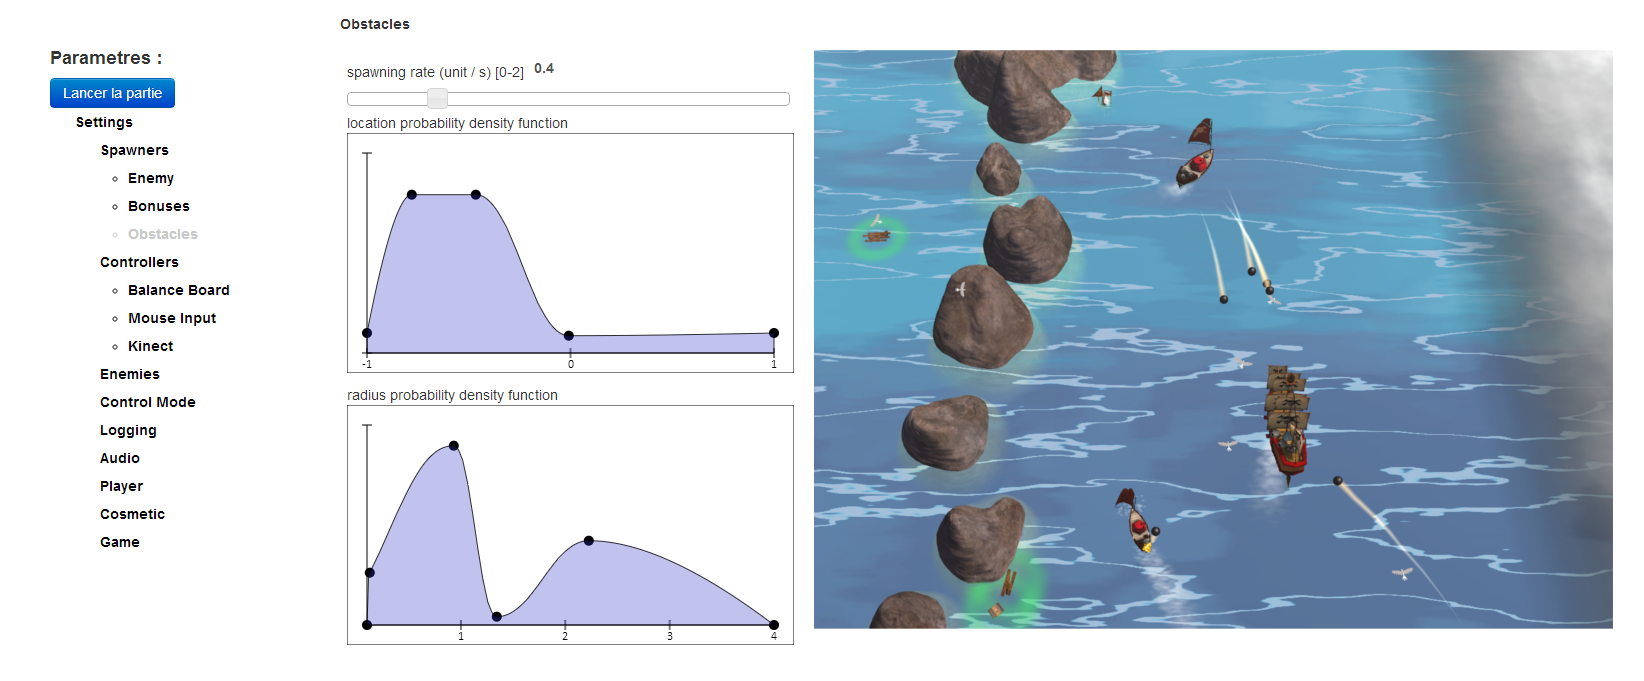
\includegraphics[scale=0.4]{images/comparatif_interface_rochers.png}
\caption{Interface thérapeutique et écran du jeu Hammer \& Planks.}
\emph{On voit que le thérapeute a changé la fonction de localisation des rochers dans l'interface, et que cela s'applique dans le jeu. Le patient est ainsi contraint de se diriger sur sa droite, l'incitant à faire travailler son coté hémiplégique.}
	\label{comparatif}
\end{figure}

\paragraph{Paramétrage des variables de jeu}
Cette partie du travail consistait en l'identification de toutes les variables dont on voudrait potentiellement modifier la valeur dans un contexte d'ajustement du jeu pour un exercice de rééducation. J'ai ensuite créé une classe spécifique permettant de regrouper conceptuellement les données modifiables. L'intérêt était que les valeurs puissent être modifiées de manière extérieure par l'interface thérapeutique. Par ailleurs, la modification de ces valeurs par l'interface devait être certaine et pérenne, afin que les modifications apportées soit effectivement prises en compte par l'application et donc modifier l'expérience de jeu en direct.

\paragraph{Usage : tests et retours\\}
Hammer \& Planks est développé en collaboration avec le service de médecine physique et de rééducation du centre hospitalier de Lapeyronie à Montpellier. Le projet a évolué et son champs d'action, en plus d'un travail sur l'équilibre, s'étend maintenant à de l'aide à la rééducation des membres supérieurs, du tronc et du bassin. Utilisant une approche de conception participative, nous avons ainsi réalisé plusieurs séances de tests avec des patients hémiplégiques et leurs thérapeutes. Ces expérimentations ont pris place au cours de plusieurs demies-journées réparties sur plusieurs mois. 

\paragraph{}
Nous avons ainsi eu de nombreux retours positifs portant sur la possibilité d'ajuster le jeu en direct, la visualisation des informations de la session de jeu ou encore le plaisir de jeu. Nous avons aussi eu de nombreuses remarques menant à l'ajout de fonctionnalités, notamment par le personnel. \\
Réaliser des tests sur des demies-journées nous a aussi permis de juger notre travail selon d'autres critères : valeurs des paramètres par défaut, robustesse de l'application sur le long terme, temps de jeu ou encore grande variabilité des profils des joueurs (personnel soignant, patients avec différentes pathologies, âge variable).

\paragraph{Conclusion\\}
Cette expérience et ce travail sur Hammer \& Planks ont permis de vérifier l'intérêt et la réelle pertinence de jeux sérieux pour la rééducation. Par ailleurs, l'intégration d'un nouveau périphérique, la Kinect, a confirmé la valeur du moyen de contrôle à la fois sur le gameplay mais aussi et surtout sur la richesse des applications thérapeutiques qui en découlent. Enfin, les critiques des soignants et des patients au cours des deux séances de tests m'ont assuré du réel intérêt de pouvoir ajuster manuellement les variables de jeux directement pendant la séance. Ceci est très encourageant pour les possibilités en terme de réhabilitation.

\paragraph{}
Cependant, un seul jeu, aussi ajustable soit il, ne peut suffire à répondre à tous les besoins et cas d'utilisation. Pour cette raison, toujours dans l'idée d'une adaptation du jeu pour le joueur-patient, la suite logique était de proposer une méthode permettant d'aider à la conception de jeux sérieux thérapeutiques.

\subsection{Aide à la conception de jeux sérieux pour la santé}
La seconde partie de mon travail fut consacrée à la proposition et à l'expérimentation de moyens de conception de jeux vidéo sérieux pour la santé. Pour cela, j'ai emprunté deux approches, répondant à des contextes un peu différents.

	\subsubsection{Ensemble d'outils d'aide à la conception de SG}
La première approche s'inscrit dans une problématique où l'on souhaite créer un serious game dont l'objectif sérieux est de l'ordre de l'aide à la réhabilitation motrice. Il s'agit ici de proposer un outil intégrant un certain nombre de connaissances utiles ou nécessaires à la conception de ce type de jeux. L'idée est de mettre à disposition des documents regroupant un maximum des informations qui seront utiles dans le processus de conception. Cela permettrait aux différents corps de métier impliqués dans le processus de conception d'avoir accès à des connaissances qui leur font défaut et d'avoir une vision globale des éléments en jeu. A la frontière entre conception de jeux vidéo et monde médical, ce travail regroupe des connaissances issues de professionnels de la santé ainsi que du domaine du jeu vidéo.

\paragraph{} On trouvera : 
\begin{itemize}
	\item un document détaillant les enjeux et objectifs thérapeutiques de la réhabilitation, particulièrement de l'AVC,
	\item une classification des objectifs thérapeutiques d'ordre moteur,
	\item une classification des principaux types de jeux vidéo,
	\item une proposition de ce que peuvent être les liens et les influences entre les éléments de différentes théories psychologiques et comportementales, notamment appliquées au contexte du serious game,
	\item une proposition de relation entre ces composantes et les objets présents dans tout jeux vidéo,
	\item une proposition de contrôles naturels pour un certain nombre de jeux vidéo grand-public existants, dans le but de leur prêter un rôle dans une rééducation fonctionnelle.
\end{itemize}
Ces documents sont tous disponibles dans le rapport de stage.

		\subsubsection{Vers une méthode de conception de SG pour la rééducation motrice}
La deuxième approche résulte en une méthode de conception basée sur une méthodologie de conception participative.

La méthode proposée ici s'inspire et conjugue les aspects les plus intéressants pour nos besoins de divers autres outils, la co-conception avec les utilisateurs restant les mots clefs de la démarche. C'est une méthode centrée sur l'utilisateur et son rôle actif dans la démarche de conception. \\
Durant mon stage, j'ai eu l'occasion de participé à la conception de plusieurs projets à divers moments du processus de conception.

\subsubsection*{Connaître Pourquoi, Qui, Comment et Quoi?}
La première étape de la démarche consiste à réunir les futurs développeurs, experts du domaine sérieux et utilisateurs de l'application afin de posséder l'intégralité des savoirs nécessaires.  On s'inspire ici de l'impact mapping pour se focaliser sur les impacts attendus de l'application.

\begin{figure}[h]
	\centering
	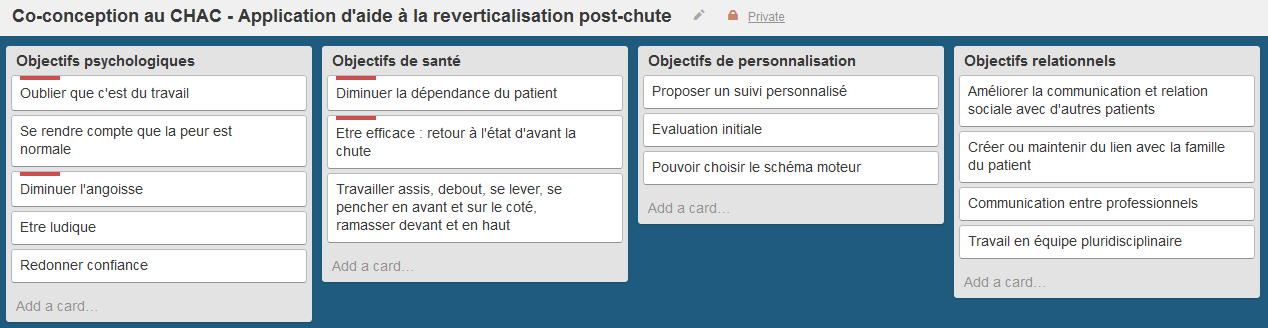
\includegraphics[width = 16cm, height=6cm]{images/objectifs_ales.png}
	\caption{Liste des objectifs issus de la séance de conception sur la verticalisation}
	\label{objectifs_ales}
\end{figure}

Pour donner un exemple, la figure \ref{objectifs_ales} donne les principaux objectifs d'une séance de conception réalisée durant mon stage. Cette séance a eu lieu au Centre hospitalier d'Alès-Cévennes. L'application envisagée a pour but d'aider des personnes, généralement âgées, étant tombées et ayant peur de rechuter, à remarcher normalement. Les objectifs marqués de rouge sont les objectifs critiques devant prioritairement être atteints. \\
On va ensuite établir les critères de réussite de ces objectifs principaux, qui permettront de vérifier de la réussite ou non du jeu sérieux qui sera créé.
 
\subsubsection*{Comprendre les utilisateurs}
On va maintenant se rapprocher des utilisateurs. Pour cela, les participants vont devoir imaginer une personne utilisatrice de l'application. Cette méthode permet de simuler un cas concret d'utilisation de l'application. Il s'agit ici de créer une carte d'empathie qui va nous permettre de dresser le profil de l'utilisateur imaginé par le groupe et de l'enrichir de toute les informations pertinentes au contexte d'utilisation de l'application à concevoir

\subsubsection*{Imaginer et illustrer les cas d'utilisation}
On va chercher à couvrir la totalité des fonctionnalités souhaitées de l'application dans différents contextes d'utilisation. Pour cela, on imagine des scénarios courts dans lesquels on pourra mettre en scène les utilisateurs imaginés lors de la séance de conception participative. \\
Ces scénarios doivent comporter trois points :
\begin{itemize}
	\item un titre : permet de rapidement cerner la fonctionnalité ou le concept illustré.
	\item une description de la scène : permet de visualiser les acteurs présents, l'action en cours et les interactions.
	\item un commentaire : permet d'expliquer ce qui se passe dans la scène, comment on en est arrivé là, les objectifs en jeux ou l'intérêt de l'application ou du jeu.
\end{itemize}

\subsubsection*{Création de storyboards}
Ils aident les utilisateurs à comprendre comment exactement l'application doit être utilisée au moyen d'une mise en scène de ces utilisations. Basés sur les scnéarios d'utilisation, c'est un moyen de personnaliser l'expérience et de rapprocher les futurs utilisateurs de l'application, en la rendant plus accessible.

\subsubsection*{Conclusion}
Cette méthode met un fort accent sur une conception collaborative de la part des différents acteurs et met l'utilisateur et les impacts au centre du processus de conception. Elle encourage des échanges réguliers entre l'équipe de développement et les utilisateurs précédemment cités, afin de vérifier que le projet reste bien en corrélation avec leurs besoins. Elle permet entre autres de partager les connaissances et les compétences des participants, ce qui contribue à la qualité globale de la conception.

\subsection{Proposition d'une nouvelle composante : La difficulté émotionnelle}
Nous avons vu dans notre recherche documentaire que sont définies trois types de difficultés dans les jeux vidéo. \cite{Levi11} définit ainsi la difficulté sensorielle, la difficulté logique et la difficulté motrice.

\paragraph{}
Il est aussi possible d'envisager une dimension émotionnelle. Celle-ci peut se manifester lors de la réalisation d'une action dont la réussite ou non est importante pour le joueur, lors d'une confrontation avec une situation, un problème ou un objet dont le joueur a peur ou le rend particulièrement mal à l'aise par exemple : mise en situation d'une phobie, d'une scène en désaccord avec ses mœurs ou convictions, scène lui rappelant des évènements difficiles ou traumatisants, etc.

\paragraph{}
Le joueur peut aussi s'imposer lui-même un certain nombre de contraintes, pour être en accord avec ses principes. Ces contraintes peuvent être d'ordre moral ou éthique (refus de tuer un personnage dans le jeu ou d'effectuer une mauvaise action), ou plus artificiel comme vouloir jouer de manière "Role Play" et donc s'interdire certaines actions ou au contraire s'en imposer d'autres.

\paragraph{Cas des serious games pour la réhabilitation motrice\\}
Dans ce cas particulier , la difficulté émotionnelle peut se situer dans l'intérêt particulier qu'a le joueur-patient dans l'évolution de sa pathologie. Il est nécessaire en phase de rééducation que le patient soit capable de sentir qu'il progresse afin de garder sa motivation et poursuive son travail. Une confrontation trop fréquente à des gestes qu'il n'est pas encore/toujours pas capable de réaliser parce que trop difficiles, aura pour conséquence de lui rappeler sa déficience et pourra lui faire perdre toute ambition thérapeutique.

\paragraph{}
Cette dernière constatation pose la question de savoir si la difficulté d'un jeu vidéo classique est comparable à celle d'un jeu thérapeutique.

%Ai-je et comment ai-je répondu à la problématique?
%1 page Perspectives
\section{Perspectives et conclusions}

\newpage
\nocite{*}
\bibliography{summary}

\end{document}